\section{Documentazione del codice}
\subsection{Strutture Dati}
Ciascuna struttura dati si ritrova all'interno del file \texttt{strutture\_dati.py}.
Le strutture dati implementate nel codice per ogni tipo di albero binario di ricerca sono le seguenti (ciascuna struttura è da considerarsi una classe):
\begin{itemize}
	\item \textbf{AlberoABR}
	\item \textbf{AlberoAVL}
	\item \textbf{AlberoRB}
	\item \textbf{Foglia}
	\item \textbf{Nodo\_ABR}
	\item \textbf{Nodo\_AVL}
	\item \textbf{Nodo\_RB}
\end{itemize}
Le classi \texttt{AlberoABR}, \texttt{AlberoAVL}, \texttt{AlberoRB} sono le classi che descrivono appunto l'albero binario di ricerca, l'albero AVL e l'albero RB.
La classe \texttt{Foglia} rappresenta il nodo sentinella \texttt{NIL},
utilizzato nelle implementazioni AVL e Rosso-Neri per rappresentare
l'assenza di nodi-figli.
Infine per ciascun tipo di albero binario di ricerca è stata fatta una classe a sè stante per ogni "tipologia" di nodo.
\subsection{Metodi}
I principali metodi che sono stati utilizzati all'interno del programma si ritrovano, come suggeriscono i nomi stessi, all'interno di ciascuna classe per ogni tipologia di albero. Essi sono i seguenti:
\begin{itemize}
	\item \textbf{Inserimento}: una volta inizializzata ciascuna tipologia di albero, si prosegue ad inserire gli eventuali nodi (sia per il caso 1 che per il caso 2). I metodi richiamano, nella loro denominazione, a quale tipo di albero fanno riferimento. Abbiamo per cui \texttt{ABR\_Tree\_Insert(z)}, \texttt{AVL\_Tree\_Insert(z)}, \texttt{RB\_Tree\_Insert(z)}. Quando il metodo viene invocato, il riferimento all'albero viene effettuato tramite \texttt{self}; $z$ è invece il nodo che viene inserito all'interno dell'albero;
	\item \textbf{Fix-Up}: I metodi di fix-up sono presenti solamente nelle implementazioni AVL e RB. Dopo un inserimento, essi risalgono il cammino dal nodo modificato verso la radice e ripristinano le proprietà di bilanciamento mediante aggiornamenti delle altezze, rotazioni e, nel caso RB, ricolorazioni. Troviamo pertanto \texttt{RB\_Insert\_Fixup(z)} e \texttt{AVL\_Insert\_Fixup(z)}. Il nodo $z$ viene distinto dal tipo di albero in esame ossia per gli AVL è il padre del nodo appena inserito; per gli alberi RB invece è il nodo che è stato appena inserito;
	\item \textbf{Rotazioni}: i metodi di Fix-up richiamano a loro volta i metodi delle Rotazioni in quanto, come detto, alberi AVL e RB usufruiscono delle rotazioni per poter ribilanciare localmente l'albero e non far violare le loro proprietà. Pertanto abbiamo \texttt{AVL\_Left\_Rotate(x)}, \texttt{AVL\_Right\_Rotate(x)}, \texttt{RB\_Left\_Rotate(x)}, \texttt{RB\_Right\_Rotate(x)}. Per ciascun metodo si ha un riferimento all'albero stesso tramite \texttt{self}, mentre $x$ è il nodo dove verrà applicata la rotazione.
\end{itemize}
\subsection{Note sul programma principale: \texttt{main.py}}
Per il programma principale sono state utilizzate librerie di Python in modo tale da:
\begin{itemize}
	\item poter generare, ai fini dell'esperimento, grafici di confronto [\texttt{matplotlib.pyplot}];
	\item misurare il tempo di esecuzione [\texttt{time}];
	\item generare valori casuali per trattare il caso casuale, corrispondente al caso medio [\texttt{random}];
	\item liberare la memoria tramite l'uso del garbage-collector [\texttt{gc}].
\end{itemize}
Sempre all'interno di \texttt{main.py}, per poter garantire la riproducibilità del caso medio, è stato fissato il $seed$ del generatore casuale al valore $42$. Conseguentemente, ad ogni esecuzione, le tre strutture ricevono la medesima permutazione casuale delle chiavi.
Inoltre il programma è stato suddiviso, sia per il caso 1 che per il caso 2 (si faccia riferimento alla sezione 2.8), in 3 parti. Pertanto si considera ciascuna azione sottostante ripetuta 2 volte:
\begin{itemize}
	\item \textbf{Inizializzazione}: ogni Albero sotto esame viene inizializzato istanziandone la classe. Vengono aggiunti 2 array per ciascun tipo di albero i quali contengono, rispettivamente, i nodi inseriti e i tempi di inserimento per ogni nodo;
	\item \textbf{Inserimento}: attraverso un parametro detto \texttt{MAX\_NODI} è possibile scegliere il numero di nodi da poter inserire all'interno di ciascun albero sia per il caso 1 che per il caso 2. Si approfondirà l'argomento nella sezione 4;
	\item \textbf{Grafici}: per entrambi i casi verranno disposti 2 grafici contenti i risultati ottenuti tramite gli inserimenti. In particolare avremmo, per ogni grafico, i tempi cumulativi di inserimento lungo le ordinate (ossia viene registrato il tempo cumulativo necessario a costruire l'albero fino a $x$ nodi) mentre lungo le ascisse avremmo il numero di nodi inseriti. Questo ci permette di poter ottenere un confronto visivo e di poter quindi constatare la teoria trattata nella sezione 2.
\end{itemize}
Una ulteriore nota, di molta importanza, fa riferimento al parametro \texttt{LIMITE}. Questo parametro è stato introdotto in quanto l'inserimento per il caso 2 poteva richiedere un grande quantitativo di tempo per poter terminare (con particolare attenzione ad un ABR generico). Questa situazione si aggravava con l'aumentare del parametro \texttt{MAX\_NODI} e pertanto la soluzione è stata quella di introdurre un limite temporale.\\ 
Questo dettaglio verrà comunque riaccennato nella sezione 4.\\ \\
Infine il \textbf{Terminale}, tramite righe di codice, permette di poter visualizzare testualmente l'andamento del programma in modo tale da tenere traccia di cosa sta succedendo prima della generazione dei grafici di confronto finali.
\subsection{Diagramma delle classi}
A seguire il diagramma delle classi: 
\begin{figure}[H]
	\centering
	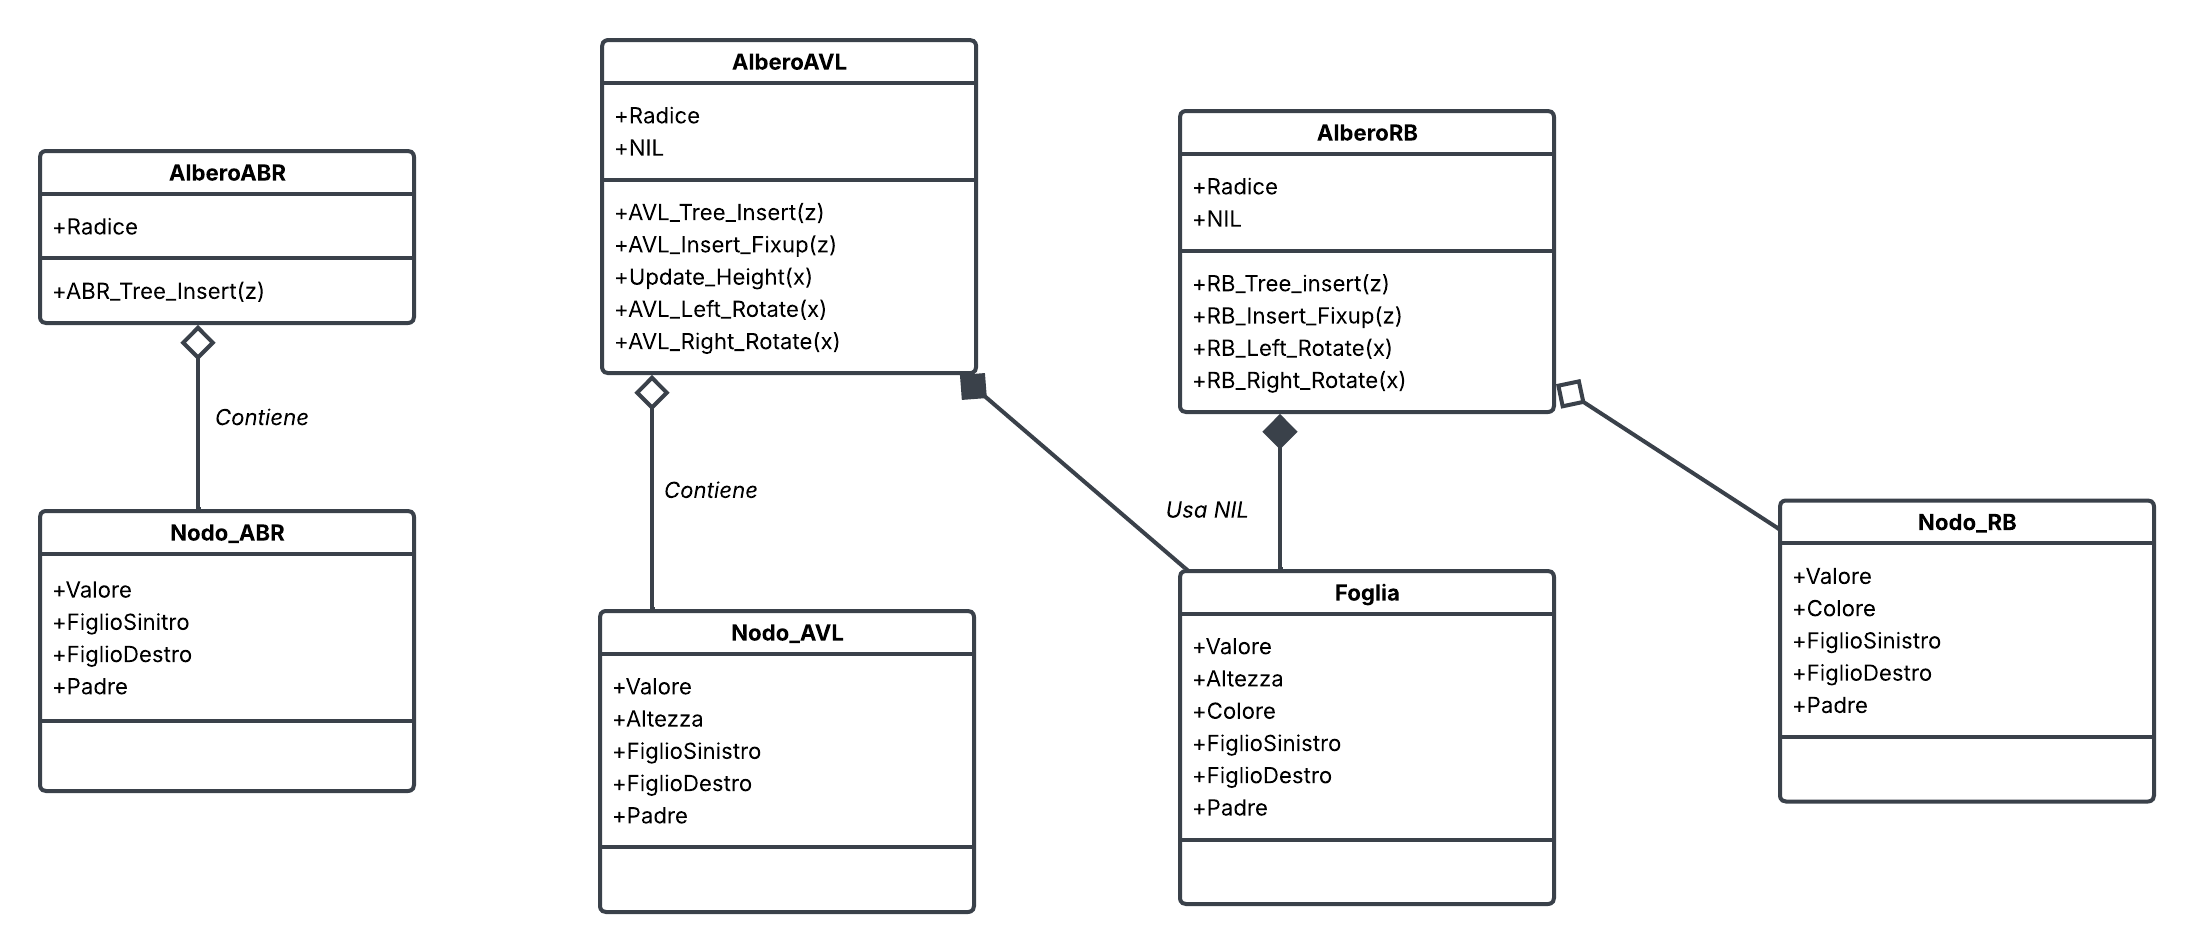
\includegraphics[width=0.9\textwidth]{Resources/UML2.png}
	\caption{Diagramma delle Classi}
	\label{fig:img}
\end{figure}
Il diagramma mostra le tre strutture principali:
\begin{itemize}
	\item \textbf{AlberoABR} contiene nodi di tipo \textbf{Nodo\_ABR};
	\item \textbf{AlberoAVL} contiene nodi di tipo \textbf{Nodo\_AVL} e usa una foglia sentinella \textbf{NIL} rappresentato dalla classe \textbf{Foglia};
	\item \textbf{AlberoRB} contiene nodi di tipo \textbf{Nodo\_RB} e usa anch'esso una foglia sentinella \textbf{NIL} della classe \textbf{Foglia}.
\end{itemize}
Le classi di "tipo" \texttt{Nodo\_X} rappresentano i singoli nodi degli alberi. Tutte possiedono attributi \texttt{Valore, FiglioSinistro, FiglioDestro, Padre}. Per nodi di tipo AVL è stato aggiunta \texttt{Altezza}, mentre per nodi di tipo RB è stato aggiunto \texttt{Colore}.
Non ci sono relazioni di ereditarietà in quanto ogni tipo di albero e ogni tipo di nodo sono implementati in classe separate. I metodi principali sono dentro le rispettive classi (in aggiunta è stato messo anche il metodo [\texttt{Update\_Height(x)}] per l'aggiornamento dell'altezza del nodo $x$ in riferimento all'albero AVL).
Infine, tramite la simbologia usata per diagrammi UML, abbiamo:
\begin{itemize}
	\item -$\lozenge$: l'albero contiene nodi;
	\item -$\blacklozenge$: l'albiero possiede il nodo sentinella \texttt{NIL}.
\end{itemize}
